\begin{appendices}
\chapter{The effect of pipeline size in regard to the time taken}
\begin{figure}[h]
\centering
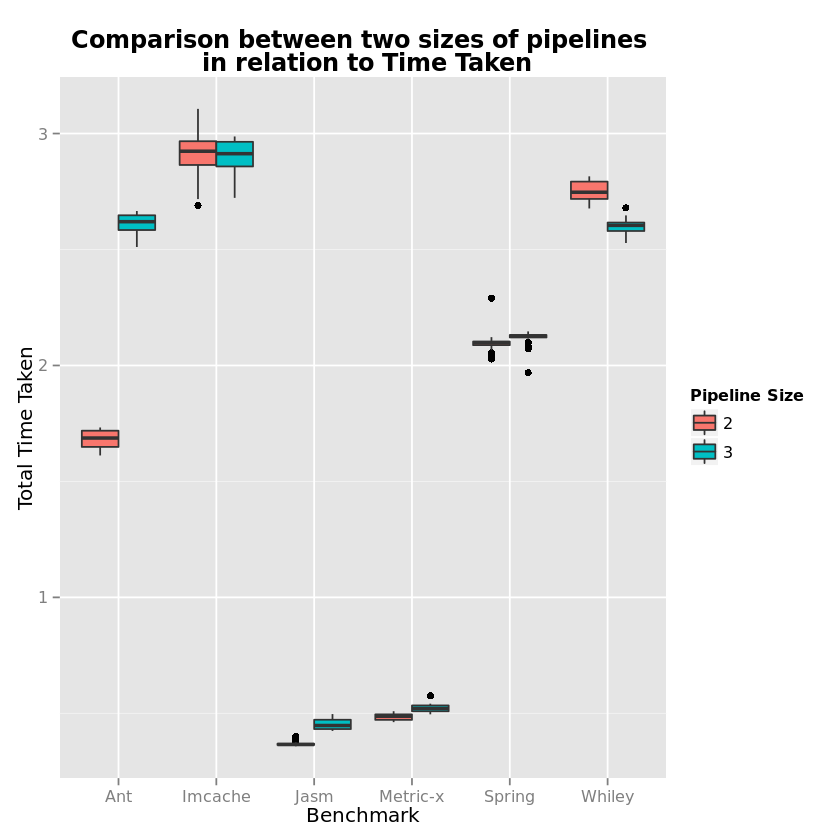
\includegraphics[width=\textwidth,height=13cm]{PipelineTime.png}
\caption{A figure showing the relationship that using different pipeline sizes has on the total time taken to analyse the data.}
\label{fig:pipelinetime}
\end{figure}

\chapter{Pipeline linear scaling}
\begin{figure}[h]
\centering
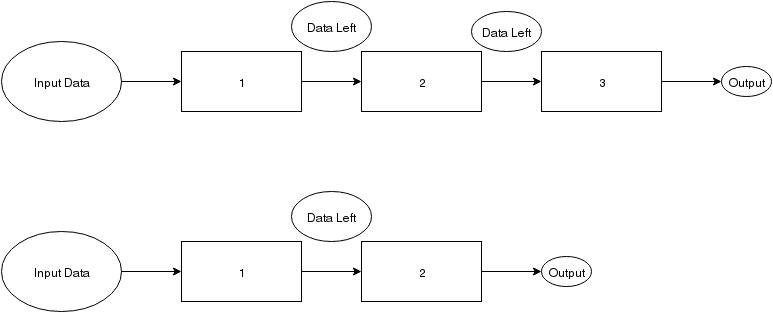
\includegraphics[width=\textwidth,height=10cm]{PipelineComp.png}
\caption{The circle size represents the data that is left in the pipeline. The figure shows that the difference that is between a two stage pipeline and a three stage only has limited room for a reduction in test cases identified. This shows that the time taken to run the extra pipeline costs more than it saves.}
\label{fig:pipelinecomp}
\end{figure}

\chapter{The effect of K Depth in regard to the time taken}
\begin{figure}[h]
\centering
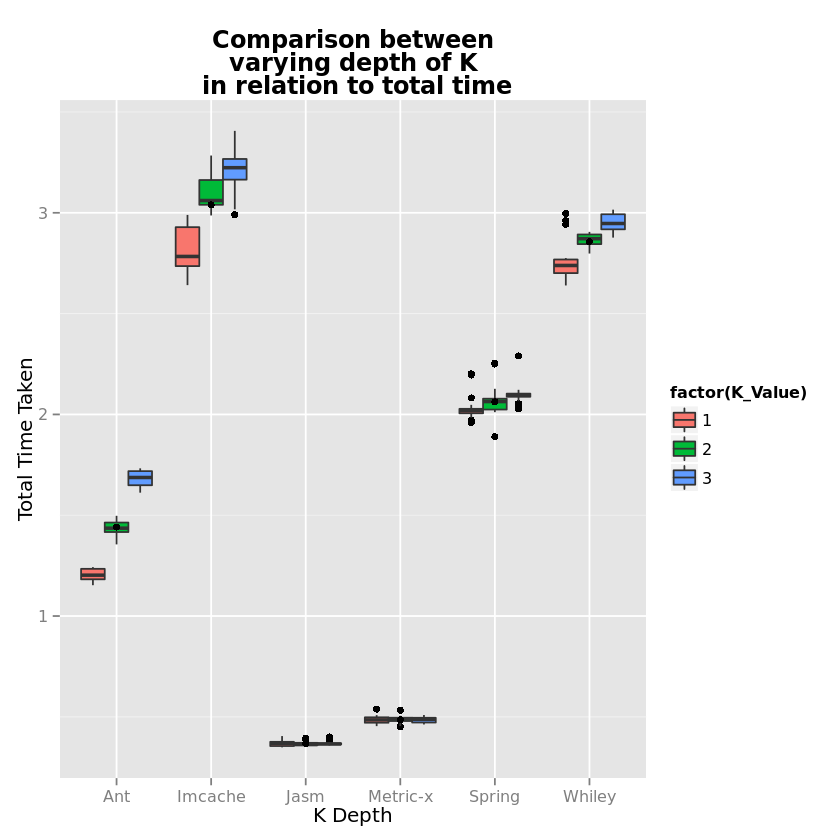
\includegraphics[width=\textwidth,height=13cm]{KDepthTime.png}
\caption{A figure showing the relationship that using a different K Depth has on the total time taken to analyse the data.}
\label{fig:kdepthtime}
\end{figure}

\chapter{The effect of parameters in regard to the time taken}
\begin{figure}[h]
\centering
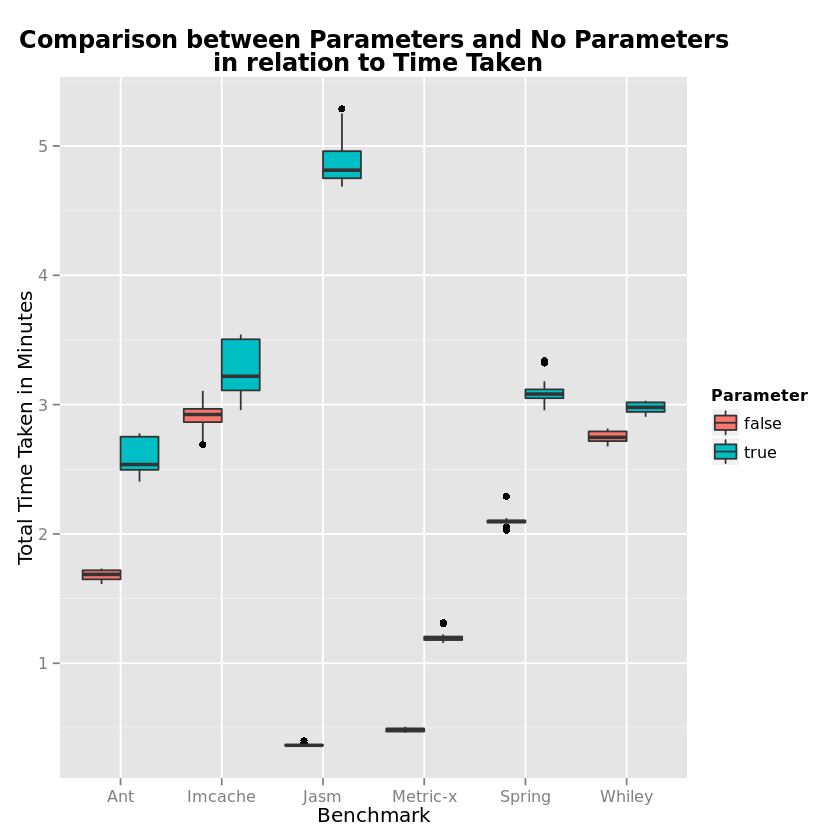
\includegraphics[width=\textwidth,height=13cm]{ParamTime.png}
\caption{A figure showing the relationship that using parameters has on the total time taken to analyse the data.}
\label{fig:paramtime}
\end{figure}

\chapter{The effect of weighting in regard to the time taken}
\begin{figure}[h]
\centering
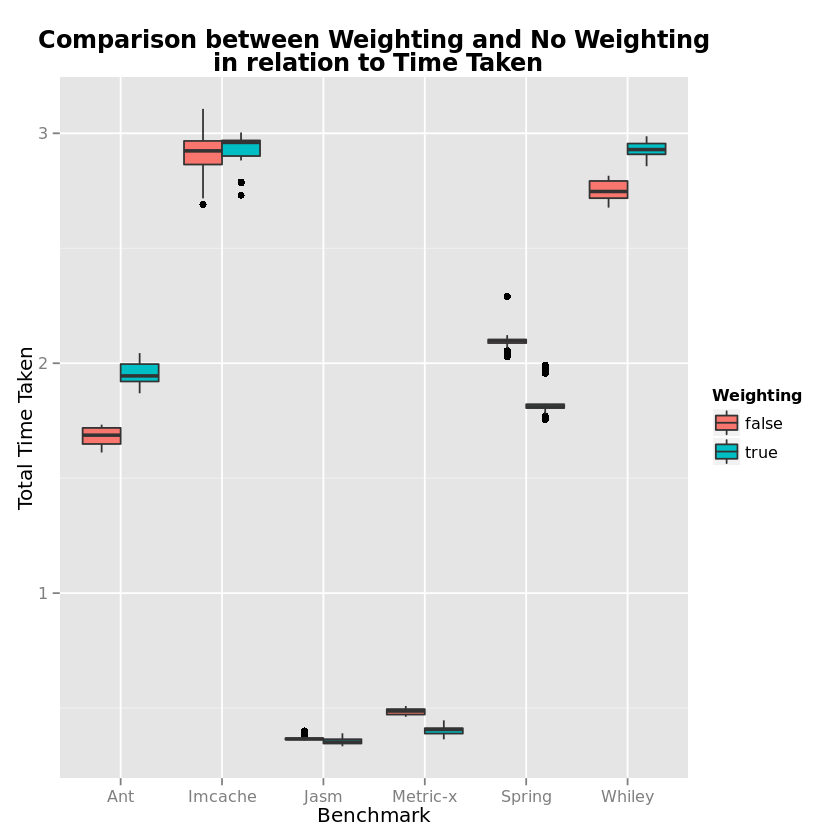
\includegraphics[width=\textwidth,height=13cm]{WeightTime.png}
\caption{A figure showing the relationship that using weighting has on the total time taken to analyse the data.}
\label{fig:weighttime}
\end{figure}

\chapter{The effect of weighting and parameters combined in regard to the time taken}
\begin{figure}[h]
\centering
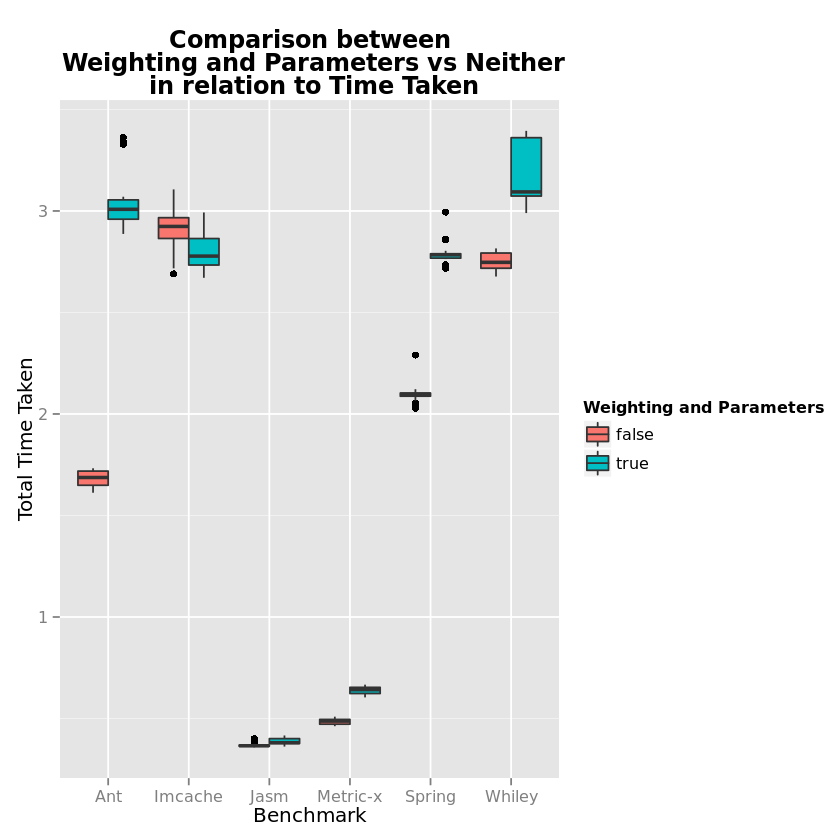
\includegraphics[width=\textwidth,height=13cm]{WeightnParamTime.png}
\caption{A figure showing the relationship that using weighting and parameters combined has on the total time taken to analyse the data.}
\label{fig:weightparamtime}
\end{figure}

\chapter{The effect of weighting and parameters vs parameters in regard to the time taken}
\begin{figure}[h]
\centering
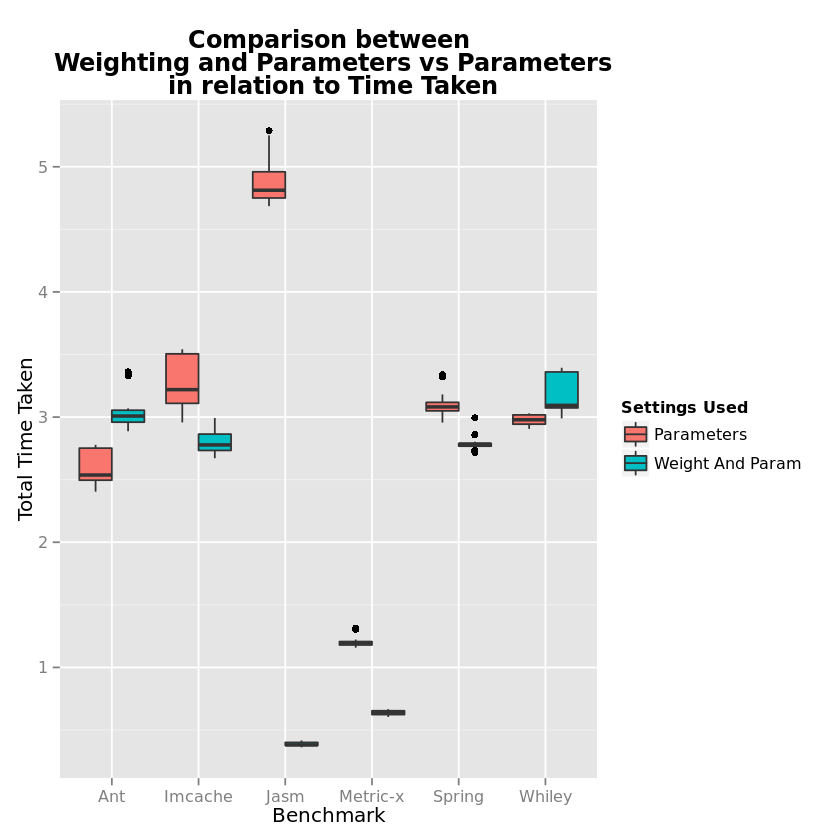
\includegraphics[width=\textwidth,height=13cm]{WeightnParamvParamTime.png}
\caption{A figure showing the relationship that using weighting and parameters combined vs parameters alone has on the total time taken to analyse the data.}
\label{fig:weightparamvparamtime}
\end{figure}




\end{appendices}